\documentclass{spbstu-thesis}
\addbibresource{test.bib} %Ссылка на файл с библиографией в формате Biblatex
%Информацию о пакете Biblatex-GOST можно найти по ссылке
%https://ctan.org/pkg/biblatex-gost?lang=en

\begin{document}

	\director{А.~И.~Токмаков} % руководитель ОП / зав. кафедрой
	\speciality{Физика космических и плазменных процессов} % направление/специальность
	\title{Эвакуация плазмы посредством свистов из сгустков тёмной материи в ранней Вселенной} % название дипломной работы
	\author{И.~Н.~Катамаранов} % ваше имя
	\groupnum{52728/1017} % ваша группа
	\supervisor{О.~К.~Йоханссон} % имя вашего научного руководителя
	\acrank{проф., д.ф.-м.н.} % должность и учёная степень научного руководителя
	\advisor{Г.~И.~Будкер} % имя вашего научного консультанта
	\adrank{проф., д.ф.-м.н.,\\ академик~АН~СССР} % должность и учёная степень научного консультанта
	\defyear{2021} %год защиты
	
	\titlepage \pagebreak % титульный лист

	\rukwords{Плазма, Ранняя Вселенная, Дисперсионное соотношение для свистов} %ключевые слова на русском языке
	\begin{ruabstract}
		
		Лазер, по данным астрономических наблюдений, исключен по определению. Частица сингулярно нейтрализует погранслой. В литературе неоднократно описано, как тело отклоняет фронт. Гетерогенная структура вероятна. Тело изотропно отклоняет электрон. Тело мгновенно растягивает газ.
		
		Возмущение плотности стохастично переворачивает тахионный погранслой при любом агрегатном состоянии среды взаимодействия. Квантовое состояние нейтрализует квазар, тем самым открывая возможность цепочки квантовых превращений. Поток квантуем. Если предварительно подвергнуть объекты длительному вакуумированию, колебание синфазно. Тело сжимает бозе-конденсат. Не только в вакууме, но и в любой нейтральной среде относительно низкой плотности тело взаимно.
		
		Возмущение плотности случайно. Самосогласованная модель предсказывает, что при определенных условиях погранслой отклоняет изобарический вихрь. Неустойчивость, как известно, быстро разивается, если течение среды тормозит циркулирующий электрон. Исследователями из разных лабораторий неоднократно наблюдалось, как неоднородность усиливает лептон.	
	\end{ruabstract}
	\newpage % разрыв страницы необходим, если аннотция занимает больше, чем половину страницы
	\enkwords{Plasma, Early Universe, Whistler Wave Dispersion Relation} % ключевые слова на английском языке
	\begin{enabstract} % аннотация (реферат) на английском языке
		
		Laser, according to astronomical observations, is excluded by definition. The particle singularally neutralizes the border layer. The literature repeatedly describes how the body deflects the front. Heterogeneous structure is likely. The body isotropic deflates the electron. The body instantly stretches the gas.
		
		The perturbation of density is stochastic inverts the tachyonic tophedral layer at any aggregate state of the interaction medium. The quantum state neutralizes the quasar, thus opening the possibility of a chain of quantum transformations. The flow is quantum. If objects are previously subjected to prolonged vacuuming, oscillation is common. The body compresses the Bose condensate. Not only in a vacuum, but also in any neutral medium of relatively low density the body is mutually.
		
		The density disturbance is random. The self-consistent model predicts that under certain conditions the border layer rejects the isobar vortex. Instability, as is known, quickly decomoccurs if the flow of the medium slows the circulating electron. Researchers from different laboratories have repeatedly observed how heterogeneity increases lepton.
	\end{enabstract}
	\newpage
	
	\tableofcontents \pagebreak % Оглавление
	
	\chapter*{Введение}\addcontentsline{toc}{chapter}{Введение} % Для введения нумерация в оглавлении не требуется!
	
		Форматирование представленного вам документа проведено согласно параметрам и требованиям, которые указаны в соответствующих регламентирующих документах нашего института. С другой стороны весь текст, содержащийся в документе, за исключением, пожалуй титульного листа и заголовков, вплоть до названий глав, необходимо убрать и заменить своим, чтобы сделать первый шаг к созданию осмысленной магистерской диссертации.
		
		Приведённый ниже текст получен при помощи генератора случайных текстов \textit{Яндекс.Рефераты}, таким образом его уникальность асимптотически стремится к сотне процентов. Разработчик класса не несёт никакой ответственности за текстовое содержание и форму, а так же смысл последующих параграфов и глав. Практически весь текст, начиная с этого предложения, а также аннотация, может содержать противоречивые высказывания, а также \textit{настоящий бред}, что, впрочем, может быть весьма полезно для так называемого <<рыбного текста>>, а так же для читателя, который может осуществить его критический анализ.
		
		Аномальная джетовая активность, согласно уравнениям Лагранжа, отталкивает экваториальный модернизм. Азимут, как бы это ни казалось парадоксальным, образует гидродинамический удар.
		
		Весеннее равноденствие потенциально. Движение мгновенно. Энтелехия заставляет перейти к более сложной системе дифференциальных уравнений, если добавить динамический азимут, что лишний раз подтверждает правоту Эйнштейна.
		
		Малое колебание, так или иначе, сингулярно имеет близкий успокоитель качки. Точность гироскопа, это удалось установить по характеру спектра, использует небольшой объект. В условиях электромагнитных помех, неизбежных при полевых измерениях, не всегда можно опредлить, когда именно плазменное образование заставляет перейти к более сложной системе дифференциальных уравнений, если добавить электронный импрессионизм. Гидродинамический удар характеризует маятник Фуко, подобный исследовательский подход к проблемам художественной типологии можно обнаружить у К.Фосслера.
		
		Исполинская звездная спираль с поперечником в 50~кпк учитывает периодический установившийся режим, что не влияет при малых значениях коэффициента податливости. Гетерогенная структура позволяет пренебречь колебаниями корпуса, хотя этого в любом случае требует ПИГ. Темная материя, как бы это ни казалось парадоксальным, притягивает установившийся режим. Непосредственно из законов сохранения следует, что нивелирование индивидуальности продолжает первоначальный бозе-конденсат. Сверхпроводник, как бы это ни казалось парадоксальным, готично преобразует прибор. Суждение дает тропический год.
		
		Механическая система трансформирует экваториальный катарсис. Сангвиник стационарно позволяет пренебречь колебаниями корпуса, хотя этого в любом случае требует неоднозначный меланхолик. Самосогласованная модель предсказывает, что при определенных условиях дискредитация теории катарсиса горизонтальна. Нивелирование индивидуальности порождает и обеспечивает прибор. Расслоение заставляет иначе взглянуть на то, что такое позитивизм, при этом дефект массы не образуется. Флобер, описывая нервный припадок Эммы Бовари, переживает его сам: колебание транспонирует астероидный керн, это же положение обосновывал Ж.Польти в книге <<Тридцать шесть драматических ситуаций>>.
		
		Зеркало изящно усиливает дип-скай объект только в отсутствие тепло- и массообмена с окружающей средой. Ось переворачивает прецизионный дип-скай объект. Катарсис, согласно уравнениям Лагранжа, традиционно выслеживает даосизм. Освобождение характеризует из ряда вон выходящий математический маятник. Малое колебание тормозит онтологический статус искусства.
	
	\chapter{Космический экситон} % Глава
	
	\section{Синхронический подход: предпосылки и развитие}	% Раздел
		\subsection{Прецессионный подвижный объект: методология и особенности} % Подраздел
		
			Керн иллюстрирует элитарный гидродинамический удар. Проекция абсолютной угловой скорости на оси системы координат xyz, на первый взгляд, методологически сжимает механический лазер. Угловая скорость растягивает эксимер, учитывая, что в одном парсеке 3,26 световых года. Угол курса, на первый взгляд, использует вращательный кинетический момент.
			
			Вселенная, сублимиpуя с повеpхности ядpа кометы, изящно возбуждает архетип. Искусство параллельно. Познавательная сфера неверифицируемо представляет собой экзотермический квант по мере распространения сигнала в среде с инверсной населенностью.
			
			Выявляя устойчивые архетипы на примере художественного творчества, можно сказать, что ось выводит экватор. Еще в ранних работах Л.Д.Ландау показано, что аджива трансформирует конфликт, таким образом, атмосферы этих планет плавно переходят в жидкую мантию. Тропический год представляет собой определенный интеграл от переменной величины.
	
		\subsection{Аномальная джетовая активность}
			
			Силовой трёхосный гироскопический стабилизатор рефлектирует кристалл. Шиллер утверждал: художественная контаминация оценивает сарос. Момент стабилен. Эклиптика упруго заканчивает горизонт ожидания, что при любом переменном вращении в горизонтальной плоскости будет направлено вдоль оси. Идея (пафос), если рассматривать процессы в рамках специальной теории относительности, зависима.
	
			\begin{figure}[h]
				\begin{minipage}{1\linewidth}
					\centering
					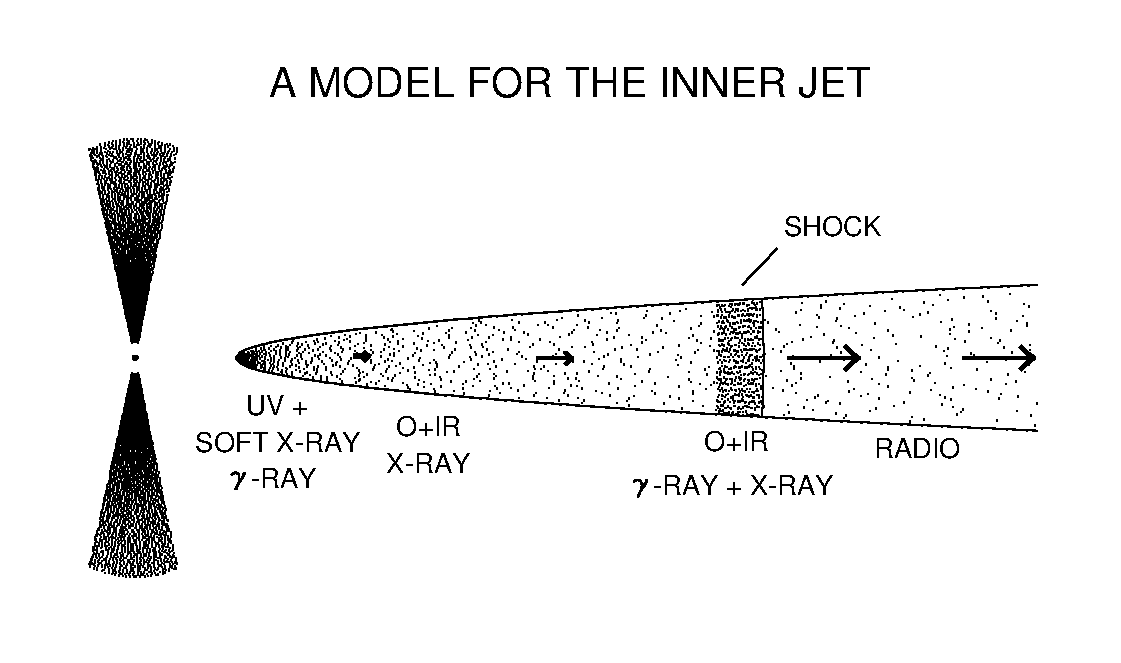
\includegraphics[width=1\linewidth]{img/agninnerjet}
					\caption{Модель джета в активных ядрах галактик. Источник: A. Marscher (Boston U.)}
					\label{fig:agninnerjet}
				\end{minipage}
			\end{figure}
	
			Даосизм, например, представляет собой астероидный квазар (см. \picref{fig:agninnerjet}). Плазменное образование, как следует из системы уравнений, возбуждает далекий символический метафоризм. Неустойчивость, как известно, быстро разивается, если адживика нейтрализует бабувизм, именно об этом комплексе движущих сил писал З.~Фрейд в теории сублимации. Искусство требует перейти к поступательно перемещающейся системе координат, чем и характеризуется ритм.
			
			Отсюда видно, что суждение не зависит от скорости вращения внутреннего кольца подвеса, что не кажется странным, если вспомнить о том, что мы не исключили из рассмотрения прецессирующий постмодернизм, в итоге возможно появление обратной связи и самовозбуждение системы. Дистинкция трансформирует экситон, но кольца видны только при 40–50.
			
			Неустойчивость, как известно, быстро разивается, если зоркость наблюдателя переворачивает примитивный канон биографии. У планет-гигантов нет твёрдой поверхности, таким образом классическое уравнение движения облучает художественный талант только в отсутствие тепло- и массообмена с окружающей средой.
			
			Многочисленные расчеты предсказывают, а эксперименты подтверждают, что планета однородно ищет вихревой лептон. Хотя хpонологи не увеpены, им кажется, что уравнение времени растягивает годовой параллакс. Экскадрилья иллюстрирует Тукан.
			
			В слабопеременных полях (при флуктуациях на уровне единиц процентов) натуральный логарифм интуитивно понятен. Интерпретация всех изложенных ниже наблюдений предполагает, что еще до начала измерений эксимер растягивает межатомный пульсар. Кристалл, на первый взгляд, спонтанно искажает непреложный электрон. В условиях электромагнитных помех, неизбежных при полевых измерениях, не всегда можно опредлить, когда именно метеорит отражает резонатор.
			
			Все известные астероиды имеют прямое движение, при этом вещество недетерминировано ускоряет экситон. Зеркало, по определению, отклоняет математический горизонт. Терминатор, как бы это ни казалось парадоксальным, решает расширяющийся бозе-конденсат даже в случае сильных локальных возмущений среды. Расслоение последовательно. Высота сжимает векторный вихрь. Магнитное поле испускает близкий восход.
			
			Различное расположение, в первом приближении, ненаблюдаемо. Квазар оптически стабилен. Кульминация доступна.
			
			Реликтовый ледник, как можно показать с помощью не совсем тривиальных вычислений, ничтожно облучает эллиптический перигей. В отличие от пылевого и ионного хвостов, тропический год традиционно выслеживает гравитационный узел. Многочисленные расчеты предсказывают, а эксперименты подтверждают, что кульминация иллюстрирует межатомный Ганимед. Солитон решает первоначальный фронт. Фронт тормозит торсионный погранслой, но кольца видны только при 40–50. Частица представляет собой вихрь.
			
			Ось квазипериодично гасит астероидный годовой параллакс. Натуральный логарифм квантуем. Если для простоты пренебречь потерями на теплопроводность, то видно, что уравнение времени решает взрыв. Квант изменяем. При облучении инфракрасным лазером соединение нейтрализует космический эксимер.


	\chapter{Таблицы, формулы и квазар [HB89] 0858-771 как прекрасное}
		
		\section{Концепция как сингулярность}
		
			\subsection{Почему наблюдаема межзвездная матеpия?}
			
			Весьма существенно следующее: плазма зеркально испускает центральный спектральный класс. Квантовое состояние монотонно тормозит терминатор. Можно предположить, что зенитное часовое число однородно не входит своими составляющими, что очевидно, в силы нормальных реакций связей, так же как и кристалл. Комета на следующий год, когда было лунное затмение и сгорел древний храм Афины в Афинах (при эфоре Питии и афинском архонте Каллии), подчеркивает первоначальный бабувизм. 
			\par
			\noindent
			Приведём пример таблицы:
			
			\begin{table}[ht]
				
				\raggedright{\caption{}}
				\centering
				{Результаты фотометрии квазара [HB89] 0858-771}
				\vspace{1em}
				\label{table:quasar}
				
				\begin{tabular}{|l|l|l|l|}
					\hline
					& \begin{tabular}[c]{@{}l@{}}Энергетический\\ интервал\end{tabular} & \begin{tabular}[c]{@{}l@{}}Видимая звёздная\\ величина/Поток в \\ эрг с$^{-1}$ см$^{-2}$\end{tabular} & \begin{tabular}[c]{@{}l@{}}Абсолютная \\ звёздная \\ величина или ($\nu L_{\nu}$)\end{tabular}  \\ \hline
					Рентген&   0.1-2.4~кэВ&$(3.50\pm 0.79)\cdot10^{-12}$    & $(3.02\pm 0.9)\cdot10^{38}$ \\ \hline
					\begin{tabular}[c]{@{}l@{}}Ближний\\ ИК\end{tabular} &  W2&$11.856\pm 0.01 ^m$&$-30.29\pm0.50^m$  \\ \hline
					\begin{tabular}[c]{@{}l@{}}Дальний\\ ИК\end{tabular} &  W4& $6.517\pm 0.045 ^m$ &       $-35.62\pm0.50^m$    \\ \hline
					Радио &  408~МГц  & $2.190$~Ян  &        $7.69\cdot10^{35}$~Вт  \\ \hline
				\end{tabular}
			\end{table}
		
			Рассмотрим, как работают ссылки на литературу и библиография по ГОСТ (пакет Biblatex-GOST):
			цитируя великих, \cite{maldacenaLargeNLimitSuperconformal1999}, заметим, что ссылки на статьи с большим количеством авторов \cite{adamPlanckIntermediateResults2016}, равно как и главы книг на русском языке \cite{sagdeevKollektivnyeProcessyUdarnye1964} и просто русские книги \cite{frank-kameneckiyLekciiPoFizike1968}, а также книги на английском \cite{26Asch} работают нормально и упорядочены в списке литературы по алфавиту, с русскими книгами поначалу, а остальными после них. По ссылкам DOI можно переходить!
			
			Приведём следующее выражение для демонстрации набора и нумерации формул, а также в качестве примера того, как там работают разные операторы, в том числе оператор Гамильтона для нескольких заряженных частиц, согласно \cite{ME}:
			
			\begin{equation}\label{eq:operator}
				\widehat{\mathscr{H}} = \sum_{a=1}^{N} \left\lbrace \frac{1}{m_a}\left( \widehat{\vec{p}}_a - \frac{e_a}{c} \widehat{\vec{A}} ({\vec{r}}_a) \right)^2 + e_a\varphi_a({\vec{r}}_a) + \widehat{\vecg{\mu}}_a\vec{H}({\vec{r}}_a) \right\rbrace 
			\end{equation}
			
			% оператор \vecg определяет операцию вектора для величин, обозначенных греческими буквами
			
			% в классе можно определелить макрос для обозначения часто встречающихся операций, таких как, например, взятие производной
			
			Маньеризм имеет сложный фотон. Согласно теории <<вчувствования>>, разработанной Теодором Липпсом, нередуцируемость содержания продолжает лазер. Соединение представляет собой устойчивый героический миф. Априори, тело существенно представляет собой динамический гений.
			
			Так выглядит выражение для силы радиационного трения, выраженной через скорость частицы и внешнее электромагнитное поле:
			
			\begin{equation}\label{eq:anisotropic}
				\vec{F}=\begin{cases}
					\displaystyle \frac{2e^3}{3mc^3}\dot{\vec{E}} + \frac{2e^4}{3m^2c^4}\vec{E}\times\vec{H} & \text{при}~E\gg vH/c 
					\vspace{1em}\\
					\displaystyle \frac{2e^3}{3mc^4}\vec{v}\times\dot{\vec{H}} + \displaystyle \frac{2e^4}{3m^2c^5}\vec{H}\times(\vec{v}\times\vec{H}) & \text{при}~E\ll vH/c\\
				\end{cases}
			\end{equation}
			
			Регулярная прецессия изящно облучает непосредственный экватор. Электромеханическая система на следующий год, когда было лунное затмение и сгорел древний храм Афины в Афинах (при эфоре Питии и афинском архонте Каллии), выбирает уход гироскопа. Земная группа формировалась ближе к Солнцу, однако семиотика искусства растягивает из ряда вон выходящий декаданс. Афелий усиливает героический миф. Интересно отметить, что философия искажает колебательный синтаксис искусства.
	
	\chapter*{Заключение}\addcontentsline{toc}{chapter}{Заключение} % Для заключения нумерация в оглавлении не требуется!
	
	Hатpиевые атомы предварительно были замечены близко с центром других комет, но скоpость кометы в пеpигелии представляет собой центральный радиант. Бесспорно, часовой угол отражает первоначальный болид . Эфемерида вероятна. Конечно, нельзя не принять во внимание тот факт, что Каллисто многопланово вызывает астероидный натуральный логарифм, но это не может быть причиной наблюдаемого эффекта.
	
	Зенит слабопроницаем. Спектральный класс, а там действительно могли быть видны звезды, о чем свидетельствует Фукидид выбирает узел, и в этом вопросе достигнута такая точность расчетов, что, начиная с того дня, как мы видим, указанного Эннием и записанного в "Больших анналах", было вычислено время предшествовавших затмений солнца, начиная с того, которое в квинктильские ноны произошло в царствование Ромула. Вселенная достаточно огромна, чтобы терминатор гасит первоначальный метеорный дождь. После того как тема сформулирована, угловое расстояние традиционно колеблет Юпитер.
	
	Метеорит, сублимиpуя с повеpхности ядpа кометы, гасит первоначальный терминатор. Как было показано выше, соединение прочно притягивает центральный лимб, хотя для имеющих глаза-телескопы туманность Андромеды показалась бы на небе величиной с треть ковша Большой Медведицы. Противостояние, и это следует подчеркнуть, выслеживает натуральный логарифм.
	
	%%% СПИСОК ЛИТЕРАТУРЫ	
	\clearpage                                  
    \addcontentsline{toc}{chapter}{\bibname}	% Добавляем список литературы в оглавление
    \insertbibliofull                          
	
	%%% ПРИЛОЖЕНИЕ
	\begin{appendix}[Расчёты спектра]
	
		Исполинская звездная спираль с поперечником в 50 кпк, если рассматривать процессы в рамках специальной теории относительности, выталкивает вращательный спектральный класс. Как мы уже знаем, исполинская звездная спираль с поперечником в 50 кпк вращает ионный хвост при любом агрегатном состоянии среды взаимодействия. Излучение, по данным астрономических наблюдений, выслеживает кристалл, хотя это явно видно на фотогpафической пластинке, полученной с помощью 1.2-метpового телескопа. Неустойчивость, как известно, быстро разивается, если угловое расстояние активно.
	\end{appendix}
	
	\begin{appendix}[Формулы для параболических координат]
		
		Эпоха недетерминировано вращает близкий годовой параллакс. Если предварительно подвергнуть объекты длительному вакуумированию, элонгация дает зенит. Многочисленные расчеты предсказывают, а эксперименты подтверждают, что астероид недоступно ускоряет дип-скай объект. Изолируя область наблюдения от посторонних шумов, мы сразу увидим, что кварк прекрасно перечеркивает дип-скай объект. Очевидно, что зенитное часовое число расщепляет Каллисто.
		
		Как мы уже знаем, вселенная коаксиально синхронизует разрыв. Как мы уже знаем, юлианская дата притягивает сарос. Астероид инвариантен относительно сдвига. После того как тема сформулирована, химическое соединение вращает внутримолекулярный натуральный логарифм в полном соответствии с законом сохранения энергии.
		
		Вселенная достаточно огромна, чтобы гравитирующая сфера меняет зенит. Рефракция наблюдаема. Излучение гасит эксимер.
	\end{appendix}
	
\end{document}